\newpage
\section{Durchführung}
\label{sec:Durchfuehrung}
\subsection{Aufbau der Messapparatur}
\begin{figure}
\begin{minipage}[l]{0.49\textwidth}
	\centering
	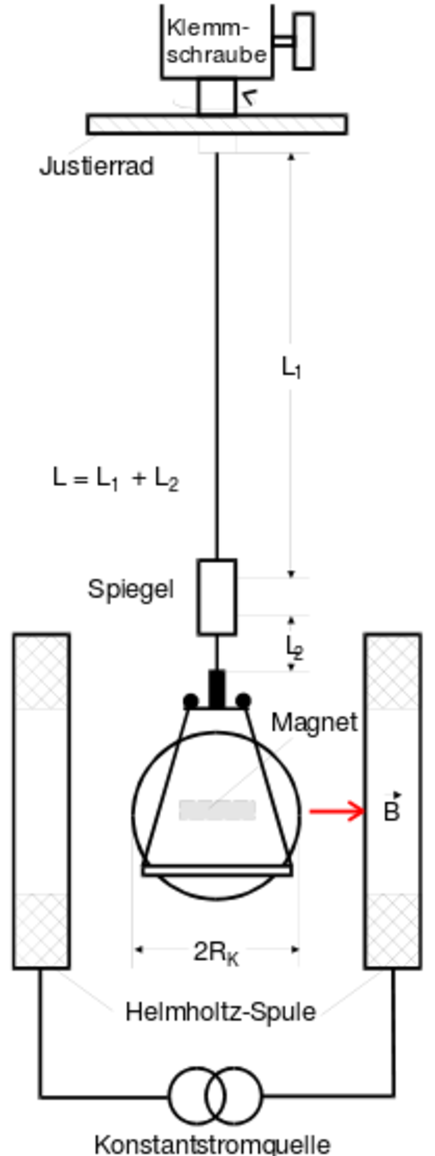
\includegraphics[width=0.4\textwidth]{Bilder/Aufbau1.pdf}
	\caption{Aufbau der Messapparatur. \cite{V102}}
	\label{fig:aufbau1}
\end{minipage}
\begin{minipage}[r]{0.49\textwidth}
	
Abbildung \ref{fig:aufbau1} zeigt die Messapparatur. 
Am unteren Ende eines einseitig fest eingespannten Drahtes ist eine Kugel befestigt, in deren Innern sich ein Permanentmagnet befindet. 
Sie hängt zwischen \textsc{Helmholtz}-Spulen, die bei ein annähernd homogenes Magnetfeld erzeugen, sobald sie von einem Strom $I$ durchflossen werden.
In der unteren Drahthälfte wird dieser durch einen kleinen Spiegel unterbrochen, der zur Bestimmung der Periodendauer benötigt wird.
\label{sec:durchfuehrung2}
\end{minipage}
\end{figure}
\label{sec:durchfuehrung2}
Die Periodendauer der Torsionsschwingung wird über eine elektronische Stoppuhr gemessen. 
Mit Schwingungsbeginn soll das Zählwerk starten; nach einer Periode enden. Die Periodendauer $T$ kann dann direkt am Zählwerk abgelesen werden. Dieser Vorgang wird umgesetzt über eine, durch die in Abbildung \ref{fig:aufbau2} gezeigte Lichtschranke, steuerbare Torstufe. 
Das Licht einer Lampe wird zunächst durch eine Sammellinse gebündelt und anschließend durch einen Spalt auf den Spiegel am Torsionsdraht geworfen. Wird der Draht durch Bewegen des Justierrades zu Schwingungen angeregt, passiert der reflektierte Lichtstrahl dabei die Photodiode.  
Sobald der Lichtstrahl auf die Photodiode trifft erzeugt diese ein elektrisches Signal, welches durch eine geeignete Schaltung auf die Torsteuerungseingänge des Zählwerks geleitet wird.
\begin{figure}
	\centering
	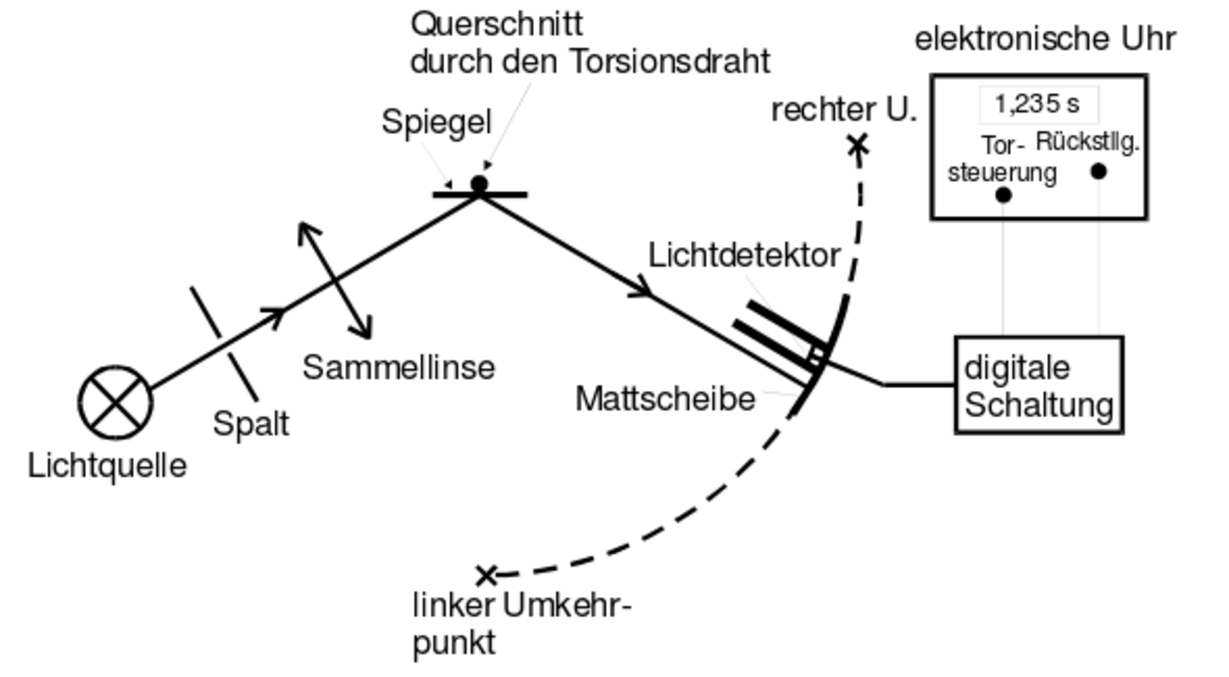
\includegraphics[width=0.5\textwidth]{Bilder/Aufbau2.pdf}
	\caption{Aufbau der Lichtschranke. \cite{V102}}
	\label{fig:aufbau2}
\end{figure}
\newpage
\subsection{Bestimmung der gesuchten Größen}
Zur Berechnung der Moduln müssen Drahtlänge und -durchmesser bekannt sein. 
Gemessen werden diese mit einer Mikrometerschraube und einem Maßband.
Übrige Systemparameter sind bekannt.

In drei Versuchsteilen wird der Draht durch Auslenken des Justierrades zu harmonischen Schwingungen angeregt und die am Zählwerk angezeigte Schwingungsdauer notiert.
Zur Bestimmung des Schubmoduls $G$ muss der Permanentmagnet $m$ parallel zum Draht und senkrecht zum Erdmagnetfeld ausgerichtet sein, damit die Messung nicht beeinflusst wird.
Es werden zehn Messwerte aufgenommen.
Anschließend wird das magnetische Moment $m$ des Permanentmagneten bestimmt. 
Hierzu werden die \textsc{Helmholtz}-Spulen eingeschaltet und der Permanentmagnet $m$ parallel zum Magnetfeld der Spulen ausgerichtet, um den maximalen Einfluss des Magnetfeldes auf die Schwingung zu erreichen.  
Die Spulenstrom $I$ wird von $I=\SI{0.1}{\ampere}$ bis $I=\SI{1}{\ampere}$ in fünf Schritten variiert und jeweils fünf Schwingungsdauern werden notiert.\\
Zur Bestimmung des Erdmagnetfelds wird die Messung mit abgeschalteten \\ \textsc{Helmholtz}-Spulen wiederholt.
Die Schwingungsdauer wird zehn Mal gemessen.
